%TCIDATA{Version=5.50.0.2960}
%TCIDATA{LaTeXparent=0,0,abowd-vilhuber-PSD-2012.tex}
                      

% $Id: main.tex 396 2013-11-03 22:29:27Z lv39 $
% $URL: https://forge.cornell.edu/svn/repos/ncrn-cornell/branches/papers/PSD2012/main.tex $
%
% main.tex

\subsection{The Curation of Confidential Data}

In the United States, the \acf{NSF} has required since January 18, 2011 that
all scientific research proposals include a detailed, viable data management
plan, thus recognizing that the acquisition, archival and curation of
scientific data is vital to the integrity of the entire process.\footnote{%
\href{http://www.nsf.gov/eng/general/dmp.jsp}{%
http://www.nsf.gov/eng/general/dmp.jsp} cited on May 20, 2012.} The relevant
test is not \textquotedblleft can the next researcher reproduce current
results,\textquotedblright\ rather it is \textquotedblleft can a researcher
working 50 or 100 years from now recover and correctly re-use the original
data.\textquotedblright\ This standard will be met when ``sufficient information exists with which to understand, evaluate, and build upon a prior work if a third party can replicate the results without any additional information from the author.''  \cite{King1995} 
Libraries have performed the curation (or
preservation) function for millennia. Social scientists recognized the
importance of data management decades ago when the \acf{ICPSR} was formed,
and again a few decades later when \ac{NSF} funded major social science data
initiatives like \ac{IPUMS} at the University of Minnesota and the \acp{RDC}
at the U.S. Census Bureau.

\ac{ICPSR} is now the largest social science data repository in the world
with over 500,000 data sets in its collection, including a growing inventory
of restricted-access datasets.\footnote{%
See \href{http://www.icpsr.umich.edu/icpsrweb/ICPSR/org/index.jsp}{%
http://www.icpsr.umich.edu/icpsrweb/ICPSR/org/index.jsp} , cited on May 20,
2012} IPUMS and IPUMS-International are the definitive sources for household
micro-data originating from population censuses around the world, including
projects for which IPUMS-International is the long-term custodian of a
foreign nation's confidential micro-data.\footnote{%
See \href{https://international.ipums.org/international/about.shtml}{%
https://international.ipums.org/international/about.shtml}, cited on May 20,
2012.} Similar archives, such as the UK Data Archive\footnote{\href{http://www.data-archive.ac.uk/about/archive}%
{http://www.data-archive.ac.uk/about/archive}, accessed May 20, 2012} and
the Australian National Data Service,\footnote{\href{http://www.ands.org.au/}%
{http://www.ands.org.au/}, accessed May 20, 2012} perform similar functions
in other countries. Within statistical agencies, researchers working at the
U.S. Census Bureau and in Census RDCs have acquired and archived a very
substantial collection of micro-data that are now used routinely for
scientific research in economics, sociology, demographics, environmental
science, health, and other fields. Other \ac{NSF}-funded efforts to make
data available have also been very successful.

Figure~\ref{fig:piechart} shows the overall distribution of data sets used
in current and historical RDC projects. It summarizes 1,505 project-dataset
pairs.\footnote{%
Many projects use multiple datasets.} %
%
% Figure Piechart (Figure 1 in NCRN proposal)
\begin{figure}[tbp]
\centering
\caption{Data sets used in U.S. Census Bureau RDC projects}
\label{fig:piechart}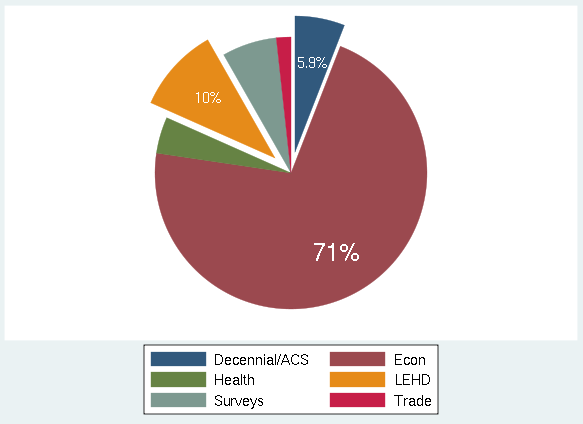
\includegraphics[width=0.5\textwidth]{pie-chart-rdc-data}
\end{figure}
Fully 71\% of all project-datasets use economic (business or establishment)
micro-data. Such data are primarily the establishment-based records from the
Economic Censuses and Surveys, the Business Register, and the \ac{LBD}. With
the exception of the recently-released Synthetic LBD \cite%
{AbowdVilhuber2010,KinneyEtAl2011}, there are no public-use micro-data for
these establishment-based products. Yet, they form the core of the modern
industrial organization studies \cite%
{DunneRobertsSamuelson1989,OlleyPakes1996} as well as modern gross job
creation and destruction in macroeconomics \cite%
{DavisHaltiwangerSchuh,HaltiwangerJarminMiranda2010}.

The next most frequently used data come from the \acf{LEHD} program, a
longitudinally integrated employer-employee database that was created
following a joint Census Bureau-NSF investment in 1999 \cite{AbowdEtAl2009}.
New confidentiality protection methodologies \cite{AbowdEtAl2012,Ashwin2008}
have unlocked large amounts of data for public-use but the structured
metadata has not kept pace. While highly detailed local area tabulations
exist based on the \ac{LEHD} data, no public-use micro-data exist for this
longitudinal job frame or any of its derivative files.

Somewhat surprisingly, only about 6\% of the project-dataset pairs involve
confidential Decennial/American Community Survey (ACS) data. Public-use
decennial files from both the long and short forms have existed for decades.
These lacked geographical detail when they were based on the old long form.
However, geographically detailed historical census and ACS files are now
part of the Census RDC-accessible micro-data collection. Thus, one can
reasonably speculate that the fraction of projects that use confidential %
\ac{ACS} will rise in the coming years.

Over the course of the last decade a framework for providing access to the
confidential micro-data that form the basis for the Census Bureau's major
data products has emerged. This framework is consistent with the statutory
obligations of the Bureau's co-custodians; namely, that research use of the
micro-data be consistent with the enabling legislation for each constituent
data source and that the appropriate administrative review occur prior to
the onset of new research. This framework is currently the best available
political compromise in the United States, but it can be considered neither
permanent nor durable.

A similar spectrum of data access protocols has emerged in Europe. They
range from relatively easy research access to confidential micro-data to
remote processing of firm or person micro-data\footnote{%
See for instance \href{http://www.bancaditalia.it/statistiche/indcamp/sondaggio/bird}%
{http://www.bancaditalia.it/statistiche/indcamp/sondaggio/bird} and \href{http://www.lisproject.org/data-access/lissy.htm}%
{http://www.lisproject.org/data-access/lissy.htm} accessed May 20, 2012.} to
simple online tabulators at most statistical agencies. As of 2012, efforts
are underway to harmonize European \cite{Bujnowska2012} or international 
\cite{Lunati2012} regulations, facilitating a standardized approach to
cross-national data access. However, it appears that most efforts have
concentrated on technical and legal questions.

To the extent that the next generations of social scientists build their
careers on the basis of original discoveries emanating from these
confidential data in the United States and elsewhere, a regulatory consensus
must emerge that treats the underlying confidential data as a vital
scientific asset, including its curation procedures.

When this consensus emerges, it will be too late to begin the curation
process. In contrast to printed data (otherwise known as books and
journals), which have unique handles (\ac{ISBN} and \ac{ISSN} are almost
universally applied), data files generally have not yet been managed in a
similar fashion.\footnote{%
To the best of our knowledge, only \ac{ICPSR} and the UK Data Archive assign
unique \acp{DOI}, but only to data that they physically control.} Part of
the problem, of course, is that while the origin and version of printed
matter used to be easily identifiable (expensive print runs and distribution
paths ensured that no book ever got to its 500th edition), data have become
more and more variable and extensible. Thus, most data currently lack a
unique handle that can be used to trace their design, provenance and vintage.

\subsection{Current Archive Model Fails}

Big data archives such as \ac{ICPSR}, \ac{IPUMS}, the UK Data Archive, or
the International Data Service Center at IZA have done an extraordinary job
of preserving public-use data--often rescuing them from oblivion--and
provide some idiosyncratic way to refer to specific samples. But there is a
fundamental, and critical, difference between the approach taken by the data
archives as compared to the approach taken by the U.S. Census Bureau, other
governmental agencies and most private organizations that use confidential
micro-data as the basis for original research or provide research access to
such data. The curation function is either absent or woefully neglected.
Consequently, there is a substantial risk of breach of the scientific
integrity of the research process itself because the findings that are
reported in the peer-reviewed journals are based on analyses of the
confidential restricted-access data, but only public-use data are released
for open scrutiny. It is the confidential data themselves that must be
curated, not just the disclosure-limited public-use products that this
research produces, in order to afford future generations of scientists the
same ability to scrutinize this work as many generations have had for work
based on the major public-use data products developed in the last 50 years.%
\footnote{%
The 1960 U.S. Census of Population and Housing Public Use Micro Sample,
released in 1963, was the first such product released by a national
statistical agency \cite{Ruggles1991}.} The statutory custodians of the
restricted-access data, in most cases government agencies but also
private-sector entities, need substantial help from the scientific community
in order to ensure that vital research data they have now acquired are
properly curated.

The problem has been caused by a subtle but pervasive barrier to effective
application of current best-practice long-term data management systems. When
conventional repositories like ICPSR, IPUMS-International and the IZA\ Data
Enclave have attempted to apply the acquisition, archive and curation
processes developed for public-use data directly to restricted-access data,
the management of restricted-access data adds an additional layer, sometimes
called stewardship, to the accepted practices. The data archive takes
physical custody of a certified-true copy of the confidential data under the
terms of a restricted-access data provider agreement with the statutory
custodian. This agreement establishes the statutory custodian's legal
authority to grant physical data custody to the archive and delineates the
terms and conditions of future use, including any disclosure limitation
protocols that must be used. At the same time, the archive acquires or
creates the metadata that are essential to the curation process. From this
point forward, management of the restricted-access data is very similar to
management of public-use data. In particular, many resources from the data
archive and the research community can be used to enhance the curation
process.

But if the conventional archive cannot take long-term custody of the
original data, this model fails because it does not have a mechanism for
synchronizing the provenance and metadata histories applicable to the
confidential data that can be audited and verified by future data users. The
U.S. Census Bureau and many other American government agencies are
prohibited by statute from granting an archive like ICPSR or IPUMS long-term
physical custody of their confidential data. Private-sector entities may
also have legal barriers emanating from data privacy promises, or may simply
hesitate to provide potential competitors access to detailed micro-data.
Both micro-data and metadata are locked up and inaccessible.

Because private entities like Microsoft or Google and government agencies
like the U.S. Census Bureau retain custody of both the confidential data and
critical metadata, a substantially modified curation protocol is required to
ensure that the actual inputs to published research are preserved. Some
requirements for this protocol are discussed here.
